% Drawing 154/09-12 -- folder 154, batch 09, archive page 168 (PDF page 169).
% Transcription: à gauche, un grand disque bordé de vert clair traversé de pseudo-droites orange, de nombreux triangles et fuseaux coloriés en jaune ; au bord, des coins marqués de traits bleus et vert foncé, étiquetés $\alpha_0$, …, $\alpha_7$, chacun deux fois, et « $\alpha_8 = \alpha_0$ » ; un arc du bord renforcé en vert foncé. À droite, une chaîne verticale de cercles au crayon enfilés sur deux pseudo-droites orange qui se tressent, avec des traits bleus aux points de passage et un gribouillis au crayon. En bas, un croisement de deux droites orange sur une droite vert clair, avec des flèches $a$, $b$ au-dessous et $a'$, $b'$ au-dessus, et une droite en tirets qui l'enjambe ; à gauche, au crayon, un fuseau étroit dans un cercle
% Kind: disk with corners alpha_0..alpha_7; chain of circles on two braided lines; crossing. Method 2 (schematic redraw from the facsimile). Status: partial.
% Notes: Skeleton. Large disk: light green rim, a dark green arc at the lower left, eight corners on the rim where two strands leave together, each with a short blue stroke and its letter (the letters are written twice at each corner on the page, once here; their order round the rim is as placed on the page view and alpha_8 = alpha_0 is not repeated), and eight strands joining the corners. The strands are indicative: they are placed from a page view with their ends on the rim, and neither their number nor the order of their crossings is that of the page; the coloured regions are not drawn. To be redrawn from a full-resolution crop. Right: five pencil circles in a vertical chain, two orange lines braided through them, crossing between consecutive circles, a blue stroke at three passages; the pencil scribble across the chain is not drawn. Bottom: two orange lines crossing on a light green line, a dashed light green line bulging over the crossing, the letters a, b below and a', b' above. Bottom left: a narrow pencil spindle with an arc. Redrawn 2026-11-12 (issue 128): to check again.
% Coordinates: 1 unit = 1 mm = 1/100 of the crop width (bbox in page fractions: [0.13, 0.075, 0.8, 0.535]).
% Redrawn by Claude (claude-fable-5-2), issue #128, 2026-11-12; not checked by a human; not compiled (no TeX in the session).
% Rights: reproduces part of the work -- behind RENDER_TRANSCRIPTS, never published by itself.
\documentclass[tikz,border=3pt]{standalone}
\usepackage{amsmath,amssymb}
\usetikzlibrary{patterns,arrows.meta}
\tikzset{Or/.style={orange!90!black}, Lg/.style={green!60!black!70}, Dg/.style={green!45!black}, Bl/.style={blue!70!black}, pencil/.style={black!45}, struck/.style={black!35}, mpt/.style={circle,draw,inner sep=1.3pt}, pt/.style={circle,fill,inner sep=0.9pt}, opt/.style={circle,draw,fill=white,inner sep=1.1pt}}
\begin{document}
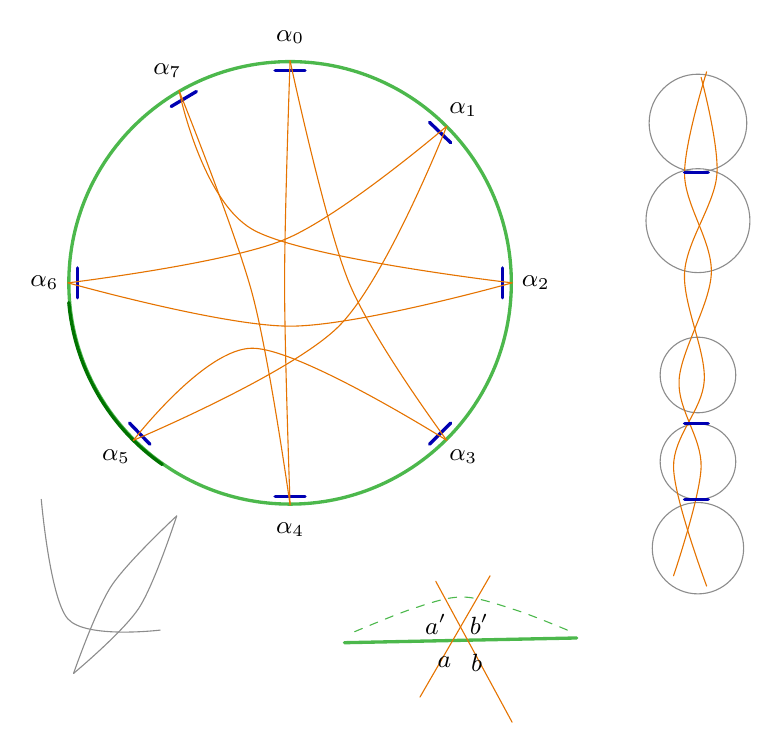
\begin{tikzpicture}[x=1mm,y=1mm,line cap=round,line join=round,font=\scriptsize]
\draw[Lg,very thick] (39.3,-36.7) circle[radius=28.1];
\draw[Dg,very thick] (11.2,-39.2) arc[start angle=185, end angle=235, x radius=28.1, y radius=28.1];
\draw[Bl,very thick] (41.2,-9.7) -- (37.4,-9.7);
\node[inner sep=1pt] at (39.3,-5.5) {\small $\alpha_0$};
\draw[Bl,very thick] (59.7,-18.9) -- (57,-16.3);
\node[inner sep=1pt] at (61.3,-14.7) {\small $\alpha_1$};
\draw[Bl,very thick] (66.3,-38.6) -- (66.3,-34.8);
\node[inner sep=1pt] at (70.5,-36.7) {\small $\alpha_2$};
\draw[Bl,very thick] (57,-57.2) -- (59.7,-54.5);
\node[inner sep=1pt] at (61.3,-58.8) {\small $\alpha_3$};
\draw[Bl,very thick] (37.4,-63.8) -- (41.2,-63.8);
\node[inner sep=1pt] at (39.3,-68) {\small $\alpha_4$};
\draw[Bl,very thick] (18.9,-54.5) -- (21.5,-57.2);
\node[inner sep=1pt] at (17.2,-58.8) {\small $\alpha_5$};
\draw[Bl,very thick] (12.3,-34.8) -- (12.3,-38.6);
\node[inner sep=1pt] at (8.1,-36.7) {\small $\alpha_6$};
\draw[Bl,very thick] (27.4,-12.4) -- (24.2,-14.3);
\node[inner sep=1pt] at (23.7,-9.7) {\small $\alpha_7$};
\draw[Or] plot[smooth, tension=0.55] coordinates {(39.3,-8.5) (38.6,-36.7) (39.3,-64.9)};
\draw[Or] plot[smooth, tension=0.55] coordinates {(39.3,-8.5) (46.8,-36.7) (59.2,-56.7)};
\draw[Or] plot[smooth, tension=0.55] coordinates {(25.2,-12.3) (34.5,-38.1) (39.3,-64.9)};
\draw[Or] plot[smooth, tension=0.55] coordinates {(59.2,-16.8) (38.6,-31.2) (11.1,-36.7)};
\draw[Or] plot[smooth, tension=0.55] coordinates {(67.5,-36.7) (39.3,-42.2) (11.1,-36.7)};
\draw[Or] plot[smooth, tension=0.55] coordinates {(67.5,-36.7) (34.5,-29.9) (25.2,-12.3)};
\draw[Or] plot[smooth, tension=0.55] coordinates {(59.2,-16.8) (45.5,-42.2) (19.4,-56.7)};
\draw[Or] plot[smooth, tension=0.55] coordinates {(59.2,-56.7) (34.5,-45) (19.4,-56.7)};
\draw[pencil] (91.1,-16.4) circle[radius=6.2];
\draw[pencil] (91.1,-28.8) circle[radius=6.6];
\draw[pencil] (91.1,-48.4) circle[radius=4.8];
\draw[pencil] (91.1,-59.4) circle[radius=4.8];
\draw[pencil] (91.1,-70.4) circle[radius=5.8];
\draw[Or] plot[smooth, tension=0.55] coordinates {(92.2,-9.9) (89.4,-23) (92.8,-35.4) (88.7,-49.1) (91.5,-60.1) (88,-73.9)};
\draw[Or] plot[smooth, tension=0.55] coordinates {(91.5,-10.6) (93.5,-23) (89.4,-35.4) (91.9,-49.1) (88,-60.1) (92.2,-75.2)};
\draw[Bl,very thick] (89.4,-22.7) -- (92.4,-22.7);
\draw[Bl,very thick] (89.4,-54.6) -- (92.4,-54.6);
\draw[Bl,very thick] (89.4,-64.2) -- (92.4,-64.2);
\draw[Lg,very thick] (46.2,-82.4) -- (75.7,-81.8);
\draw[Lg,dashed] plot[smooth, tension=0.55] coordinates {(47.5,-81) (55.1,-78) (61.3,-76.6) (68.1,-78.3) (75,-81)};
\draw[Or] (55.8,-89.3) -- (64.7,-73.9);
\draw[Or] (57.8,-74.6) -- (67.5,-92.5);
\node[inner sep=1pt] at (58.9,-84.9) {\small $a$};
\node[inner sep=1pt] at (63,-84.9) {\small $b$};
\node[inner sep=1pt] at (57.8,-80.1) {\small $a'$};
\node[inner sep=1pt] at (63.3,-80.1) {\small $b'$};
\draw[pencil] plot[smooth, tension=0.55] coordinates {(11.8,-86.3) (16.6,-75.2) (24.9,-66.3)};
\draw[pencil] plot[smooth, tension=0.55] coordinates {(11.8,-86.3) (20.1,-78) (24.9,-66.3)};
\draw[pencil] plot[smooth, tension=0.55] coordinates {(7.7,-64.2) (11.1,-79.4) (22.8,-80.8)};
\end{tikzpicture}
\end{document}
